% This is samplepaper.tex, a sample chapter demonstrating the
% LLNCS macro package for Springer Computer Science proceedings;
% Version 2.20 of 2017/10/04
%
\documentclass[runningheads]{llncs}
%
\usepackage{graphicx}
% Used for displaying a sample figure. If possible, figure files should
% be included in EPS format.
%
% If you use the hyperref package, please uncomment the following line
% to display URLs in blue roman font according to Springer's eBook style:
% \renewcommand\UrlFont{\color{blue}\rmfamily}

\begin{document}
%
\title{An Event-based Architecture for Multi-population Optimization Algorithms}
%
%\titlerunning{Abbreviated paper title}
% If the paper title is too long for the running head, you can set
% an abbreviated paper title here
%
\author{Erick Vargas Minguela\inst{1}\orcidID{0000-1111-2222-3333} \and
Mario Garcia Valdez\inst{1}\orcidID{1111-2222-3333-4444} \and
Third Author\inst{2}\orcidID{2222--3333-4444-5555}}
%
\authorrunning{E. Vargas Minguela et al.}
% First names are abbreviated in the running head.
% If there are more than two authors, 'et al.' is used.
%
\institute{National Technological Institute of Mexico 
\email{erick.vargas.minguela@gmail.com}\\
%\url{http://www.springer.com/gp/computer-science/lncs}\\
\email{\{abc,lncs\}}}
%
\maketitle              % typeset the header of the contribution
%
\begin{abstract}
  % It seems like the abstract is incompleate, it is a good idea to 
  % write it at the end - Mario 
    This article explains about an architecture designed to create an easy way to
    distribute the processing of population-based algorithms with the idea of avoiding 
    getting stuck in a value looking for a solution of a combinatorial problem, creating 
    multiple fragments from a single population with different
    parameters of execution, also this feature allows to hybridate different techniques by adding multiple algorithms,
     in this case it is implemented with Genetic Algorithms (GA) and Particle Swarm Optimization (PSO). 
    Having the knowledge that both of them are population-based algorithms it
    can be defined that a migration between 2 or more populations are possible,
    and this type of hybrid could be helpful to increase the possibility to find the
    optimal result (the best of the best), there is where fits the concept of
    Multi-population. For this type of work we used asynchronous functions,
    serverless functions, multithread and a distributed architecture taking
    advantage of functional programming and serverless architecture. Even
    nature works like that... parallel, asynchronous and distributed.



\keywords{Multi-population  
  \and Asynchronous 
  \and Sub-population 
  \and Serverless 
  \and Distributed.}
\end{abstract}
%
%
%
\section{Introduction}
A universe of solutions can exist for a single optimization problem and sometimes
is too big and complex to solve it in a traditional way. That is why heuristic and
population-based algorithms are required. % They are just one of the options. -
Mario This kind of algorithms are very useful to solve combinatory problems,
however, usually one is better than others to solve one thing and another is
great to solve another problem, and there are several cases stucked in optimal
local values. % Add a bit more detail - Mario

In this work, we propose an architecture composed by serverless functions to
create a multi-populations that will process sub-populations in distributed
function architecture and they are going to be parallel and asynchronous making
each sub-population distributed and independent. And comunicating using
migrations to help each other preventing fall into optimal local values. % the
sentence is a bit confusing - Mario
% Add a connection between the previous idea (multi-algorithms,
% multi-populations) with distributed and serverless.

Distributed and cloud-based architectures are used extensivly in the software
industry because of their high performance and lower overall cost.  Many systems
are being created and migrating step by step to microservices and... in a nearly
future... the new architectures called serverless, which proposes the use of
“Function as a Service” (FaaS).
% I think you are not finished writing the above sentence. - Mario

\subsection{Serverless}
Recently, the cloud providers as Amazon Web Services (AWS), Google Cloud, etc.
Offers a new alternative to programming throught interfaces called Serverless
Computing, this kind of platform consist in a very simple mecanism where the
developer upload the code into the platform and execute it as mamy times it is
required scalling and allowing do this in a parallel way. This way the
developers do not worry about servers, connections and other configurations. In
serverless it pays only for what is used. Even there are some platform that
allows to install them into your own server to do your own local architecture
serverless.

\begin{figure}[htp]
  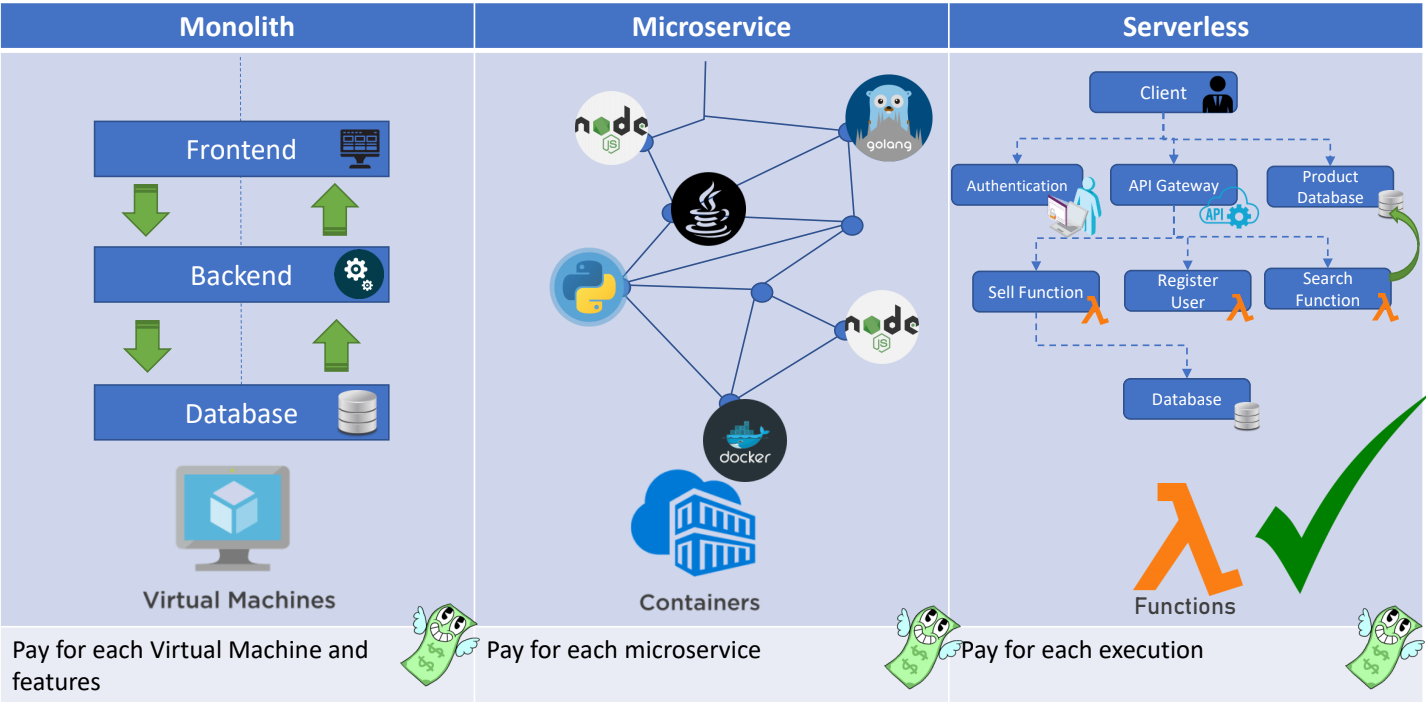
\includegraphics[width=\textwidth]{img/architectures.png}
  \caption{Software architecture generations.} \label{fig1}
  \end{figure}

\subsubsection{Serverless Function} 
In math a function is a relation between a set of inputs and an allowed set of
outputs with the idea that each input goes to a single output. But in computer
science is small bits of code that do only one thing and are easily to
understand and support. In serverless this functions could be triggered by an
event that would be menssages, http request,etc. Also is known that each
function scales independently and is stateless with a short duration.


\section{Proposed architecture}

The propose is an architecture that allows to process a simple population that
is divided into sub-populations distributing them to process in different ways
and then communicating each other with purpose of increase the possibility to
find the best fitness of a function. This architecture can accept the use of an
indeterminate number of algorithms, allowing an easy hybridation and continuous
adaptability for different problems.

This architecture consist in 3 nodes, they are explained on the next points:

\begin{itemize}
  \item Manager: Here the multi-population is managed, it is initialized how to
  process it, followed by the subpopulations, which when they are concepted
  trigger an event that sends the subpopulations to be stored in a file JSON of
  MongoDB (preventing to saturate the memory) and to a message queue that is
  directed to its subsequent processing in the “Receiver” section that is our
  cluster of functions (Faas), because each subpopulation requires the execution
  of a different algorithm, there is a different channel in the web sockets for
  each type of algorithm that triggers its respective serverless function. Once
  a subpopulation is processed, it is returned and a selection is made for the
  sub-population migration. The migration selection is made by taking the
  population attribute of the subpopulation that was returned and the
  subpopulation that it have been selected among the best 2, it should be noted
  that the decision to identify the best from the 2 is made randomly. Once the
  selection is made, a Splitting Point Uniform crossing will be made. The 2 new
  subpopulations replace their self and are resent it back to their respective
  serverless function and this process is repeited until completing the number
  of assigned migrations for the multi-population. Of course this whole process
  is performed asynchronously avoiding wait for all responses from serverless
  functions to perform a crossover or a update of the multi-population status
  \cite{Lovbjerg2001,Jimeno2019}. In the following figure you can see from
  illustrative way how the multi-population is composed.
\begin{figure}[htp]
  \centering
  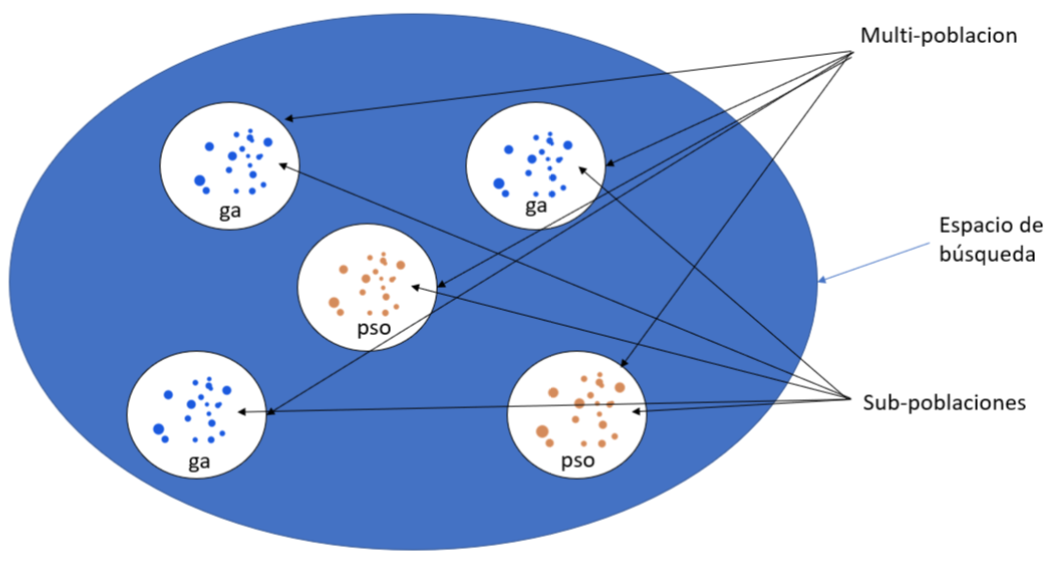
\includegraphics[width=0.7\textwidth]{img/multipopulation.png}
  \caption{Multipopulation representation.} \label{fig1}
  \end{figure}
\item Message Provider: Its purpose is the creation of a sub-population messages
queue which is the comunication channel between the sub-population Manager and
the Receiver (FaaS), each message is a trigger for the execution of a GA or PSO
function. Thanks to the message queue, it is possible to perform the serverless
functions asynchronously, avoiding that the algorithm wait for responses
independently of their duration and the simultaneous evaluation of different
sub-populations independent of its algorithm or characteristics.
\item Receiver: The following section contains the Serverless functions of the
algorithms to be executed, reduced the best possible using the functional
programming paradigm so that they can be converted into FaaS without problems,
in addition to achieving a completely clean and fast execution
\cite{Roberts2016} . Each message received on this node is executed in the form
of a multi-threaded process in parallel, this allows to having more than one
population-based search algorithm running at the same time, and making a copy of
itself each algorithm function as required.
\end{itemize}

To develop this architecture the applied technologies are based in JavaScript
using Node JS as it can be see it in the General Architecture Flowchart.

\begin{figure}[htp]
  \centering
  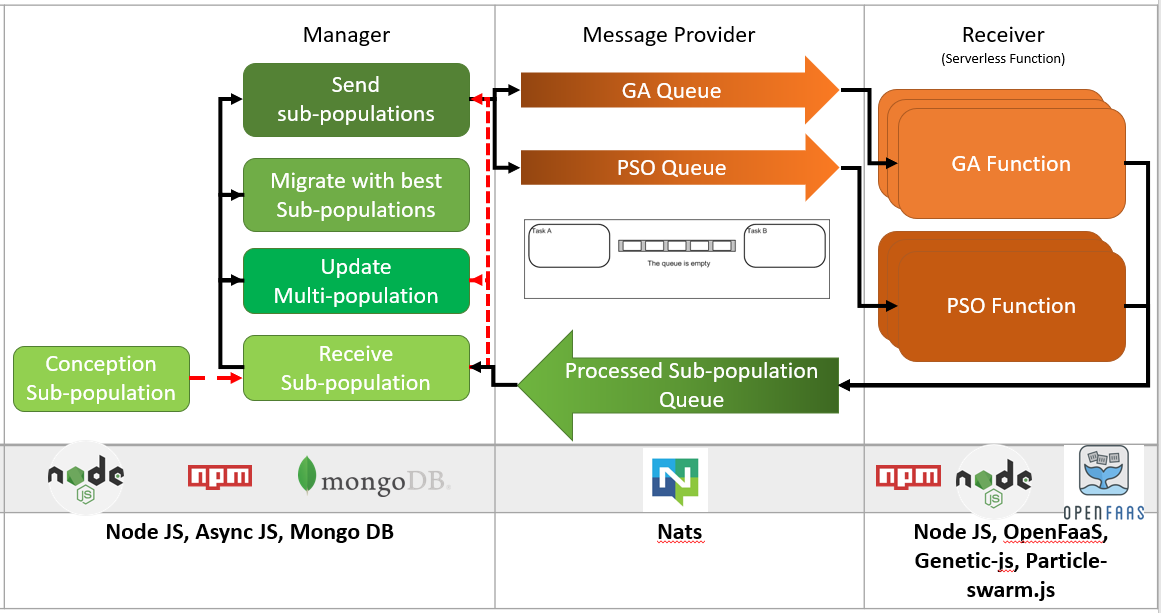
\includegraphics[width=0.9\textwidth]{img/general diagram architecture 2.png}
  \caption{General Architecture Flowchart.} \label{fig1}
  \end{figure}

\subsection{Sub-population definition}

Individuals are created composed of 2 types of information, the one that is
active or useful for crossing and the one that is not. The population contains
the series of possible solutions, while the rest contains the information on how
the processing for the search of the optimal solutions will be executed, linked
directly with their respective algorithms.

\begin{figure}[htp]
  \centering
  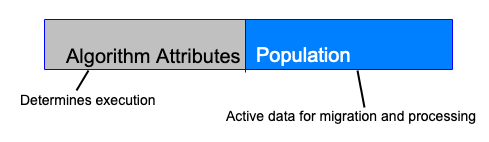
\includegraphics[width=0.6\textwidth]{img/subpopulationDefinition.png}
  \caption{Sub-population composition.} \label{fig1}
  \end{figure}

\subsection{Splitting Point Uniform Migration}
A uniform mask is created to apply the migration between individuals from 2
sub-populations. The selected data are combined using the middle point between
the selected points by the mask. This process iterates the 2 sub-populations to
randomly swap values and replace some of them with middle points.


\begin{figure}[htp]
  \centering
  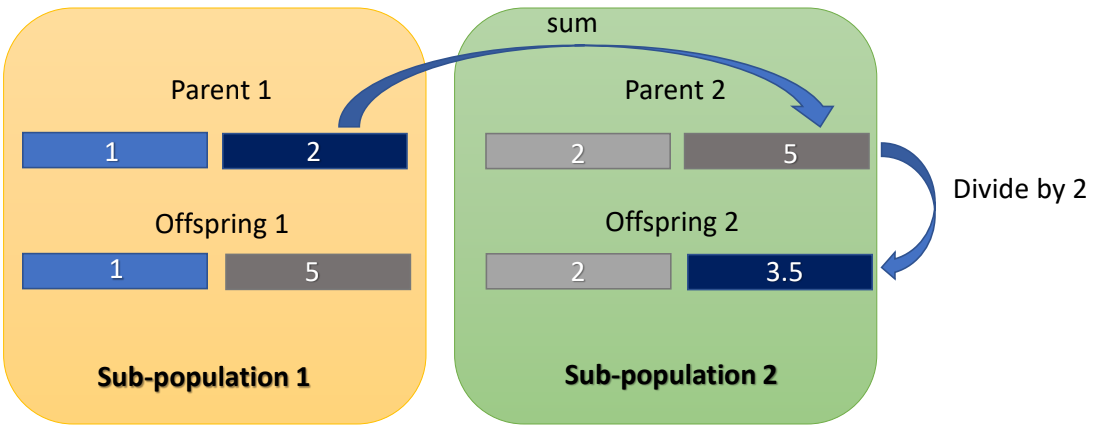
\includegraphics[width=0.9\textwidth]{img/splittinPointUniform.png}
  \caption{Splitting Point Uniform process.} \label{fig1}
  \end{figure}

  \subsection{Migration Selection}

  Using migration selection by tournament keeping up the information of the best
  sub-population of the multi-population.

\begin{figure}[htp]
  \centering
  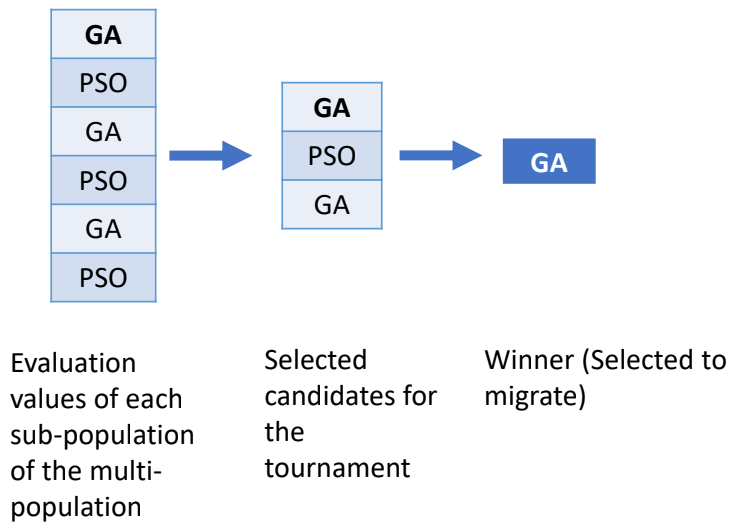
\includegraphics[width=0.5\textwidth]{img/selection.png}
  \caption{Selection by tournament.} \label{fig1}
  \end{figure}


\section{Experiments and Results}
\subsection{Experiments}
Now that an interaction between sub-populations with different algorithms it is
working and  hybridation have been a success, using until now the added
algorithms (GA and PSO) algorithms, all thanks to the developed architecture,
lets procede to the experiments. This section is going to be the execution of
several experiments from 2 to 40 dimensions, with a stop criterial of an error
below  0.5E-8, without a parameter optimization method, waiting that the
architecture by its self would be enough to increase the possibility to find a
better optimal result than the traditional methods. All this hoping that the
results will probe the needness of this kind of architecture on increasing
dimensions. To test if the architecture was useful, several experiments were
made to solve benchmark functions, for this case the functions are Sphere,
Rastrigin and Rosenbrock. Using 10 sub-population for each experiment and
maximum 4 migrations per sub-population with different algorithms and parameters
for each sub-population.

\begin{figure}[htp]
  \centering
    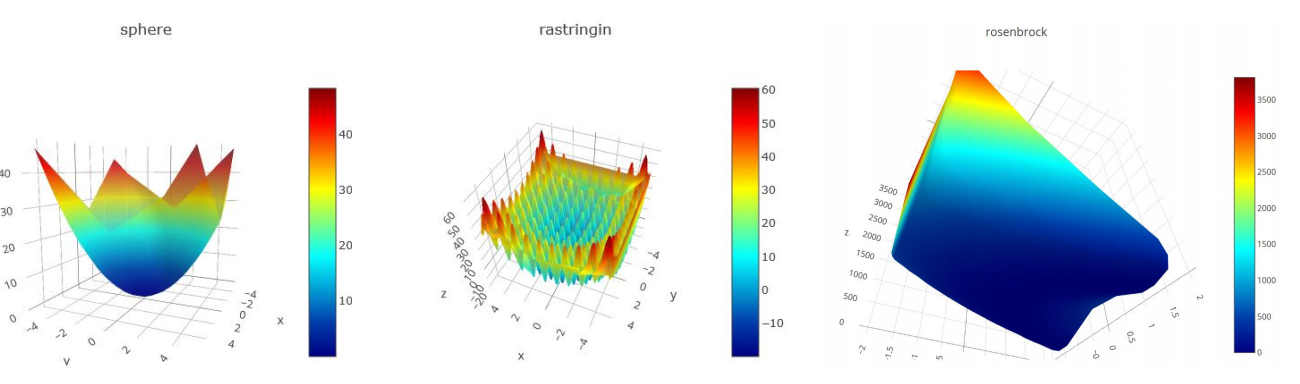
\includegraphics[width=0.7\textwidth]{img/benchmark.png}
    \caption{Benchmark functions for experimentation.} \label{fig1}
    \end{figure}

\subsection{Parameters Configuration} 

This architecture modifies the traditional way to work with population based
algorithms, then the experiments could not be parameterized as usually are.

Then the experiments are scaled by their number of evaluations and the
parameters must be configured to be adjusted to the next criterial, using the
next expression:

\begin{equation}
    \label{eq:hesitancy-interpretation}
   Evaluations = 10^{5} Dimensions
   \end{equation}

For example, if the experiment has 2 dimensions, the maximum number of
evaluations will be 200,0000, for 10 dimensions will be 1,000,000 of evaluacions
and the same with the others dimensions.









   \begin{table}[htp]
    \caption{2 dimension parameters}
    \label{table:ga-pso-parameters-2}
    \centering
    \begin{tabular}{|l|l|}
    \hline
    Parameter & Value \\
    \hline
    \hline
    GA Optimization & Minimize \\
    \hline
    GA Generations & 50 \\
    \hline
    GA Dimensions & 2 \\
    \hline
    GA Population size & 100 \\
    \hline
    GA Mutation & Random(Tournament2,Tournament3,Random \\
    &  ,RandomLinearRank,Sequential,Fittest)\\
    \hline
    GA Crossover & Tournament3 \\
    \hline
    GA Crossover percentage & Random[10\%, 80\%] \\
    \hline
    GA Mutation percentage & Random[10\%,50\%] \\
    \hline
    GA Crossover function & Uniforme de punto medio \\
    \hline
    GA Mutation Function & gaussian \\
    \hline
    PSO Optimization & Minimiza \\
    \hline
    PSO Iterations & 50 \\
    \hline
    PSO Dimensions & 2 \\
    \hline
    PSO Vector size & 100 \\
    \hline
    PSO Social factor & Random[0.5,4.0] \\
    \hline
    PSO Individual factor & Random[0.5,4.0] \\
    \hline
    PSO Inercia factor & Random[0.5,4.0] \\
    \hline
    \end{tabular}
    \end{table}

\begin{figure}[htp]
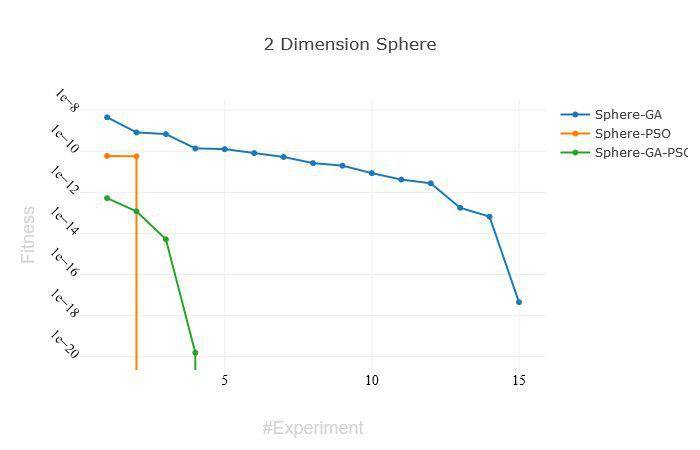
\includegraphics[width=\textwidth]{img/2-sphere.jpg}
\caption{2 dimension experiments Sphere.} \label{fig1}
\end{figure}

\begin{figure}[htp]
  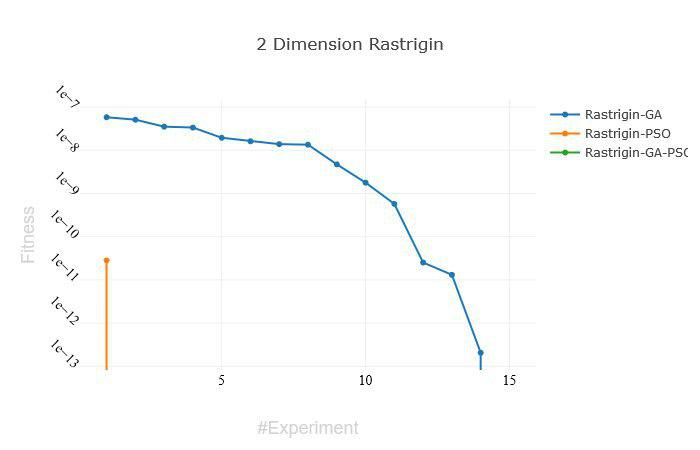
\includegraphics[width=\textwidth]{img/2-rastrigin.jpg}
  \caption{2 dimension experiments Rastrigin.} \label{fig1}
  \end{figure}
  
\begin{figure}[htp]
  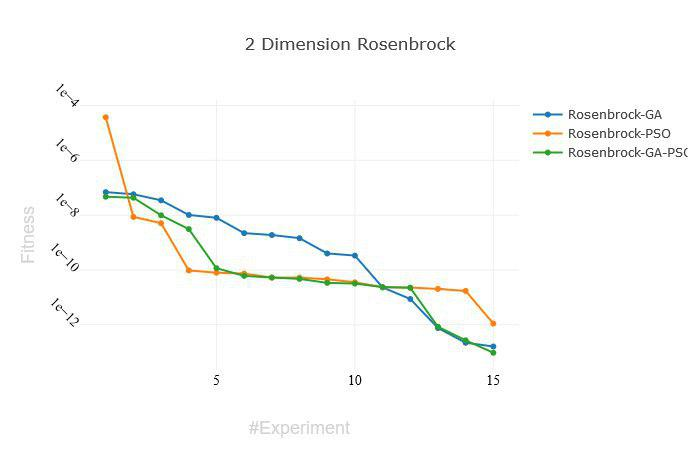
\includegraphics[width=\textwidth]{img/2-rosenbrock.jpg}
  \caption{2 dimension experiments Rosenbrock.} \label{fig1}
  \end{figure}

\begin{table}[htp]
    \caption{2 dimensional experiment results}
    \label{table:resultados-2}
    \centering
    \begin{tabular}{|c|c|c|c|}
    \hline
    Fn & Best & AVG & Experiment Number \\
    \hline
    \hline
    Rastrigin GA & 0 & 1.65377E-08 & 15\\
    \hline
    Rastrigin PSO & 0 & 1.8872E-12 & 15\\
    \hline
    Rastrigin GA-PSO & 0 & 0 & 15\\
    \hline
    Sphere GA & 4.53222E-18 & 4.36977E-10 & 15\\
    \hline
    Sphere PSO & 0 & 7.8012E-12 & 15\\
    \hline
    Sphere GA-PSO & 0 & 4.33161E-14 & 15\\
    \hline
    Rosenbrock GA & 1.62335E-13 & 1.24176E-08 & 15\\
    \hline
    Rosenbrock PSO & 1.11674E-12 & 2.47795E-06 & 15\\
    \hline
    Rosenbrock GA-PSO & 9.5809E-14 & 6.90695E-09 & 15\\
    \hline
    \end{tabular}
    \end{table}
  
    \begin{table}[htp]
      \caption{10 dimensions parameters}
      \label{table:ga-pso-parameters-10}
      \centering
      \begin{tabular}{|l|l|}
      \hline
      Parameter & Value \\
      \hline
      \hline
      GA Optimization & Minimiza \\
      \hline
GA Generations & 70 \\
      \hline
GA Dimensions & 10 \\
      \hline
GA Population size & 200 \\
      \hline
GA Mutation & Random(Tournament2,Tournament3,Random \\
      &  ,RandomLinearRank,Sequential,Fittest)\\
      \hline
GA Crossover \\
      \hline
GA Crossover percentage & Random[10\%, 80\%] \\
      \hline
GA Mutation percentage & Random[10\%,50\%] \\
      \hline
GA Crossover function & Uniforme de punto medio \\
      \hline
GA Mutation Function & gaussian \\
      \hline
PSO Optimization & Minimiza \\
      \hline
PSO Iterations & 70 \\
      \hline
PSO Dimensions & 10 \\
      \hline
PSO Vector size & 200 \\
      \hline
PSO Social factor & Random[0.5,4.0] \\
      \hline
PSO Individual factor & Random[0.5,4.0] \\
      \hline
PSO Inercia factor & Random[0.5,4.0] \\
      \hline
      \end{tabular}
      \end{table}
    
      \begin{figure}[htp]
        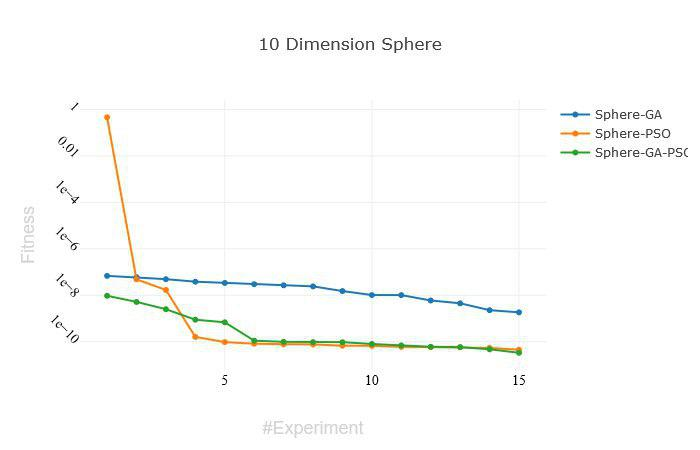
\includegraphics[width=\textwidth]{img/10-sphere.jpg}
        \caption{10 dimensions experiments Sphere.} \label{fig1}
        \end{figure}

        \begin{figure}[htp]
          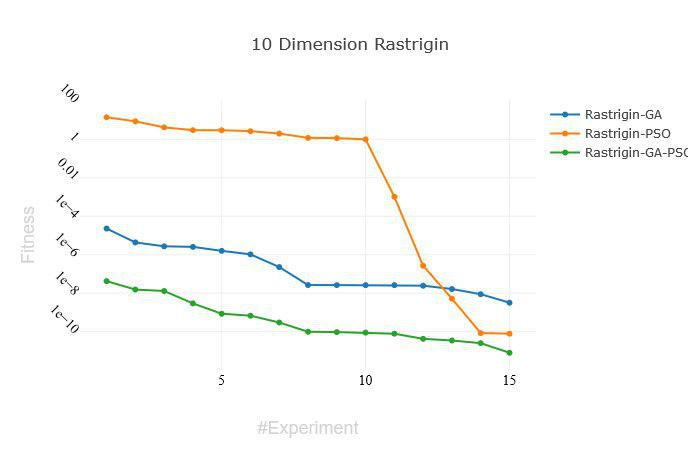
\includegraphics[width=\textwidth]{img/10-rastrigin.jpg}
          \caption{10 dimensions experiments Rastrigin.} \label{fig1}
          \end{figure}

          \begin{figure}[htp]
            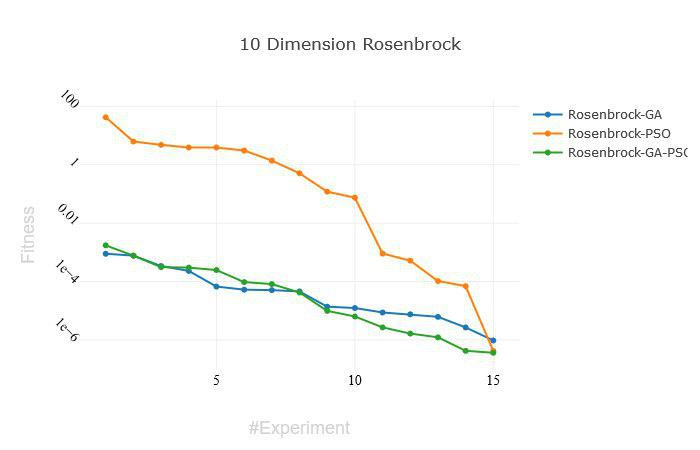
\includegraphics[width=\textwidth]{img/10-rosenbrock.jpg}
            \caption{10 dimensions experiments Rosenbrock.} \label{fig1}
            \end{figure}

        \begin{table}[htp]
          \caption{10 dimensional experiment results}
          \label{table:resultados-2}
          \centering
          \begin{tabular}{|l|l|l|l|}
          \hline
          Fn & Best & Average & Experiment Number \\
          \hline
          \hline
          Rastrigin GA & 3.21768E-09 & 2.38015E-06 & 15\\
          \hline
          Rastrigin PSO & 7.8586E-11 & 2.715716161 & 15\\
          \hline
          Rastrigin GA-PSO & 8.01492E-12 & 5.08668E-09 & 15\\
          \hline
          Sphere GA & 1.84051E-09 & 2.5389E-08 & 15\\
          \hline
          Sphere PSO & 4.50351E-11 & 4.72855E-09 & 15\\
          \hline
          Sphere GA-PSO & 3.33851E-11 & 1.30062E-09 & 15\\
          \hline
          Rosenbrock GA & 9.58323E-07 & 1.24176E-08 & 15\\
          \hline
          Rosenbrock PSO & 4.16711E-07 & 4.431565444 & 15\\
          \hline
          Rosenbrock GA-PSO & 3.62472E-07 & 0.000240251 & 15\\
          \hline
          \end{tabular}
          \end{table}

          \begin{table}[htp]
            \caption{Parametros experimentos 20 dimensiones}
            \label{table:ga-pso-parameters-20}
            \centering
            \begin{tabular}{|l|l|}
            \hline
            Parameter & Value \\
            \hline
            \hline
            GA Optimization & Minimiza \\
            \hline
            GA Generations & 70 \\
            \hline
            GA Dimensions & 20 \\
            \hline
            GA Population size & 200 \\
            \hline
            GA Mutation & Random(Tournament2,Tournament3,Random \\
            &  ,RandomLinearRank,Sequential,Fittest)\\
            \hline
            GA Crossover & Tournament3 \\
            \hline
            GA Crossover percentage & Random[10\%, 80\%] \\
            \hline
            GA Mutation percentage & Random[10\%,50\%] \\
            \hline
            GA Crossover function & Uniforme de punto medio \\
            \hline
            GA Mutation Function & gaussian \\
            \hline
            PSO Optimization & Minimiza \\
            \hline
            PSO Iterations & 70 \\
            \hline
            PSO Dimensions & 20 \\
            \hline
            PSO Vector size & 200 \\
            \hline
            PSO Social factor & Random[0.5,4.0] \\
            \hline
            PSO Individual factor & Random[0.5,4.0] \\
            \hline
            PSO Inercia factor & Random[0.5,4.0] \\
            \hline
            \end{tabular}
            \end{table}
          
            \begin{figure}[htp]
              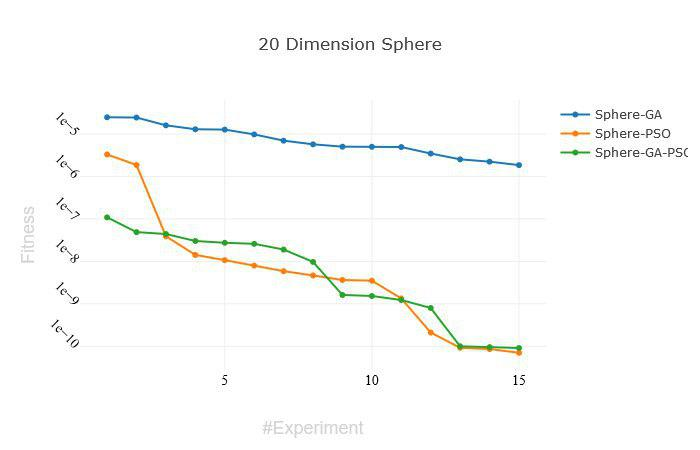
\includegraphics[width=\textwidth]{img/20-sphere.jpg}
              \caption{20 dimensions experiments Sphere.} \label{fig1}
              \end{figure}
      
              \begin{figure}[htp]
                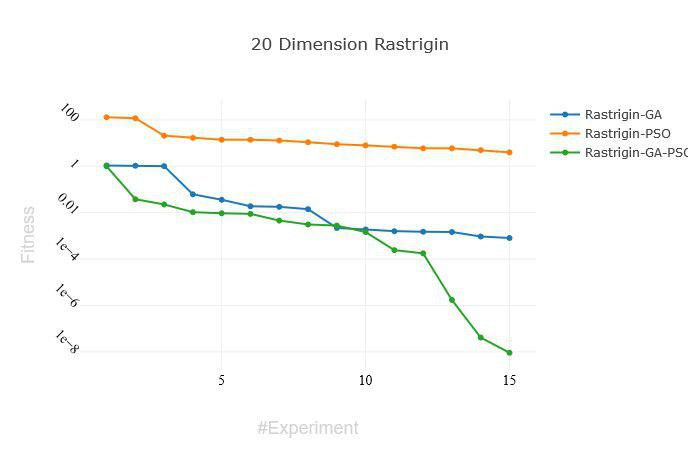
\includegraphics[width=\textwidth]{img/20-rastrigin.jpg}
                \caption{20 dimensions experiments Rastrigin.} \label{fig1}
                \end{figure}
      
                \begin{figure}[htp]
                  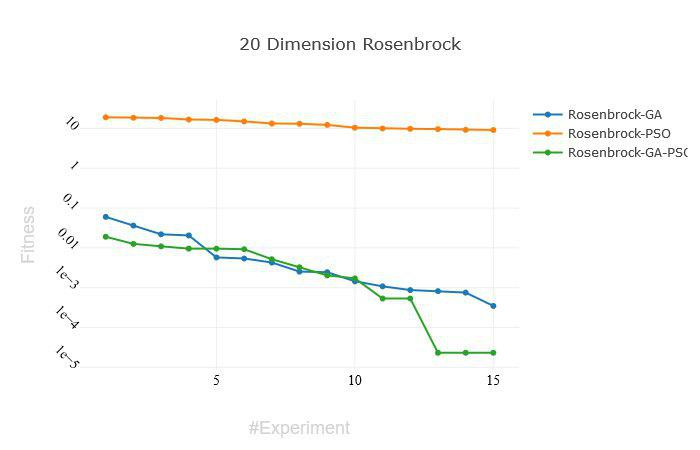
\includegraphics[width=\textwidth]{img/20-rosenbrock.jpg}
                  \caption{20 dimensions experiments Rosenbrock.} \label{fig1}
                  \end{figure}

                  \begin{table}[htp]

    \caption{Resultados 20 dimensiones}
    \label{table:resultados-2}
    \centering
    \begin{tabular}{|l|l|l|l|}
    \hline
    Fn & Best & Average & Experiment Number \\
    \hline
    \hline
    Rastrigin GA & 0.000808633 & 0.220596203 & 15\\
    \hline
    Rastrigin PSO & 3.988070734 & 25.51777514 & 15\\
    \hline
    Rastrigin GA-PSO & 9.13E-09 & 7.38E-02 & 15\\
    \hline
    Sphere GA & 1.84051E-09 & 9.22715E-06 & 15\\
    \hline
    Sphere PSO & 7.04E-11 & 3.50E-07 & 15\\
    \hline
    Sphere GA-PSO & 9.11E-11 & 2.13E-08 & 15\\
    \hline
    Rosenbrock GA & 0.000348015 & 0.010958941 & 15\\
    \hline
    Rosenbrock PSO & 9.119539342 & 13.37613983 & 15\\
    \hline
    Rosenbrock GA-PSO & 2.31663E-05 & 0.005608855 & 15\\
    \hline
    \end{tabular}
    \end{table}

    \begin{table}[htp]
      \caption{Parametros experimentos 40 dimensiones}
      \label{table:ga-pso-parameters-20}
      \centering
      \begin{tabular}{|c|c|}
      \hline
      Parameter & Value \\
      \hline
      \hline
      GA Optimization& Minimiza \\
      \hline
      GA Generations & 70 \\
      \hline
      GA Dimensions & 40 \\
      \hline
      GA Population size & 200 \\
      \hline
      GA Mutation & Random(Tournament2,Tournament3,Random \\
      &  ,RandomLinearRank,Sequential,Fittest)\\
      \hline
      GA Crossover \\
      \hline
      GA Crossover percentage & Random[10\%, 80\%] \\
      \hline
      GA Mutation percentage & Random[10\%,50\%] \\
      \hline
      GA Crossover function & Uniforme de punto medio \\
      \hline
      GA Mutation Function & gaussian \\
      \hline
      PSO Optimization & Minimiza \\
      \hline
      PSO Iterations & 70 \\
      \hline
      PSO Dimensions & 40 \\
      \hline
      PSO Vector size& 200 \\
      \hline
      PSO Social factor & Random[0.5,4.0] \\
      \hline
      PSO Individual factor & Random[0.5,4.0] \\
      \hline
      PSO Inercia factor & Random[0.5,4.0] \\
      \hline
      \end{tabular}
      \end{table}
    
      \begin{figure}[htp]
        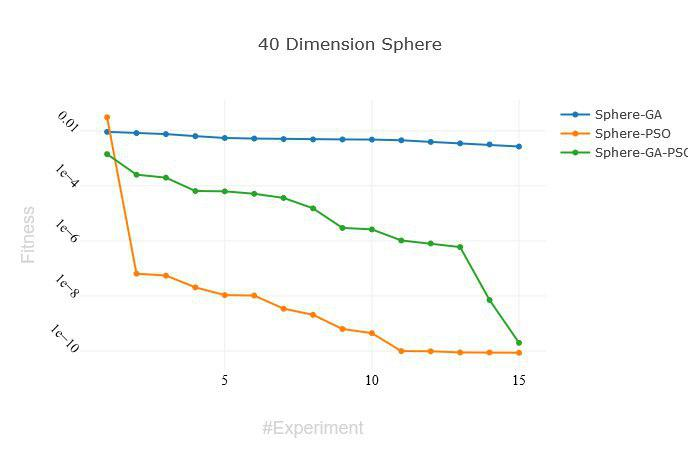
\includegraphics[width=\textwidth]{img/40-sphere.jpg}
        \caption{40 dimensions experiments Sphere.} \label{fig1}
        \end{figure}

        \begin{figure}[htp]
          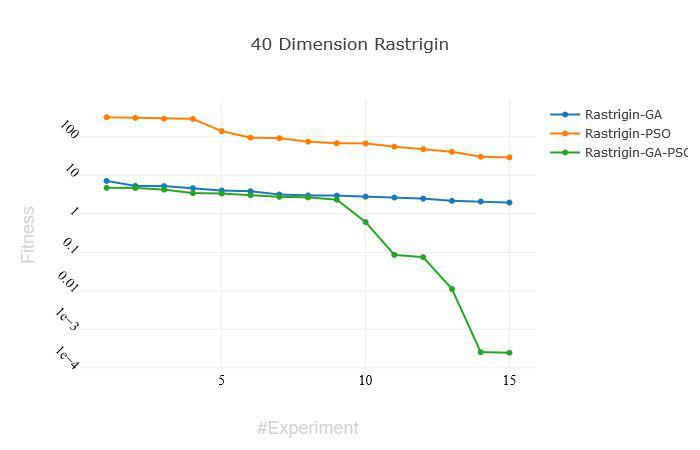
\includegraphics[width=\textwidth]{img/40-rastrigin.jpg}
          \caption{40 dimensions experiments Rastrigin.} \label{fig1}
          \end{figure}

          \begin{figure}[htp]
            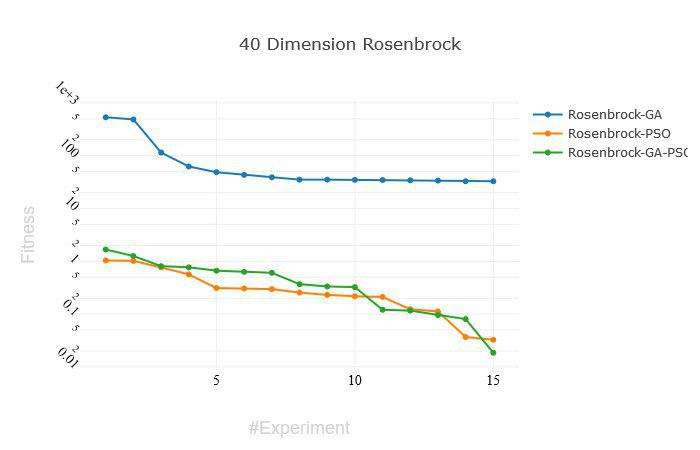
\includegraphics[width=\textwidth]{img/40-rosenbrock.jpg}
            \caption{40 dimensions experiments Rosenbrock.} \label{fig1}
            \end{figure}

            \begin{table}[htp]
              \caption{Resultados 40 dimensiones}
              \label{table:resultados-2}
              \centering
              \begin{tabular}{|l|l|l|l|}
              \hline
              Fn & Best & Average & Experiment Number \\
              \hline
              \hline
              Rastrigin GA & 1.95478879 & 3.560837088 & 15\\
              \hline
              Rastrigin PSO & 29.06596132 & 130.2865863 & 15\\
              \hline
              Rastrigin GA-PSO & 2.46E-04 & 2.13E+00 & 15\\
              \hline
              Sphere GA & 0.002686956 & 0.005302951 & 15\\
              \hline
              Sphere PSO & 8.68E-11 & 2.07E-03 & 15\\
              \hline
              Sphere GA-PSO & 2.00E-10 & 1.41E-04 & 15\\
              \hline
              Rosenbrock GA & 0.000348015 & 106.9287542 & 15\\
              \hline
              Rosenbrock PSO & 0.032708559 & 0.368395353 & 15\\
              \hline
              Rosenbrock GA-PSO & 0.018538924 & 0.525086565 & 15\\
              \hline
              \end{tabular}
              \end{table}
% ---- Bibliography ----
%
% BibTeX users should specify bibliography style 'splncs04'.
% References will then be sorted and formatted in the correct style.
%
% \bibliographystyle{splncs04}
% \bibliography{mybibliography}
%
\section{Conclusion}

This architecture is completely scalable and useful for hybridation of multiple algorithms,
until now is only GA and PSO but according with the results with this kind of architecture
there is no limit and it works better than multi-populations with only one algorithm, also
every experiment executes in short times because serverless functions searching in an asynchronous way getting a fast convergence.

\section{Future work}

To get a continuous improvement it is believed that it is required a sort of mutation applied to the 
sub-populations. This mutation would be a swapping type, taking the algoritm parameters from the best and the worst 
sub-populations, increasing the possibilities to get and optimal result, preventing get stucked into a local optimum.
Of course it is expected to use this architecture using more algorithms than GA and PSO.


\bibliography{samplepaper}
      \bibliographystyle{ieeetr}
  %  \begin{thebibliography}{10}
      
    % \bibitem{Hellerstein2018}
    % J.~M. Hellerstein, J.~Faleiro, J.~E. Gonzalez, J.~Schleier-Smith, V.~Sreekanti,
    %   A.~Tumanov, and C.~Wu, ``{Serverless Computing: One Step Forward, Two Steps
    %   Back},'' vol.~3, 2018.
    
    % \bibitem{Kramer2017}
    % O.~Kramer, ``{Genetic Algorithm Essentials},'' {\em Springer International
    %   Publishing AG}, vol.~679, pp.~11--20, 2017.
    
    % \bibitem{Guerrero2017}
    % C.~Guerrero, I.~Lera, and C.~Juiz, ``{Genetic Algorithm for Multi-Objective
    %   Optimization of Container Allocation in Cloud Architecture},'' {\em Journal
    %   of Grid Computing}, pp.~1--23, 2017.
    
    % \bibitem{Lalwani2019}
    % S.~Lalwani, H.~Sharma, S.~Chandra, S.~Kusum, D.~Jagdish, and C.~Bansal,
    %   ``{REVIEW - COMPUTER ENGINEERING AND COMPUTER SCIENCE A Survey on Parallel
    %   Particle Swarm Optimization Algorithms},'' {\em Arabian Journal for Science
    %   and Engineering}, 2019.
    
    % \bibitem{Blum2005}
    % S.~Blum, R.~Puisa, and M.~Wintermantel, ``{Adaptive Mutation Strategies for
    %   Evolutionary Algorithms},'' {\em 2nd Weimar Optimization and Stochastic
    %   Days}, pp.~1--13, 2005.
    
    % \bibitem{Everywhere}
    % S.~Everywhere, ``{The Fn Project},''
    
    % \bibitem{Ma2019}
    % H.~Ma, S.~Shen, M.~Yu, Z.~Yang, M.~Fei, and H.~Zhou, ``{Multi-population
    %   techniques in nature inspired optimization algorithms : A comprehensive
    %   survey},'' {\em Swarm and Evolutionary Computation}, vol.~44, no.~July 2017,
    %   pp.~365--387, 2019.
    
    % \bibitem{Santander-jim2018}
    % S.~Santander-jim and M.~A. Vega-rodr, ``{Comparative Analysis of
    %   Intra-Algorithm Parallel Multiobjective Evolutionary Algorithms : Taxonomy
    %   Implications on Bioinformatics Scenarios},'' vol.~9219, no.~c, pp.~1--15,
    %   2018.
    
    % \bibitem{Sherry2012}
    % D.~Sherry, K.~Veeramachaneni, J.~McDermott, and U.~M. O'Reilly, ``{Flex-GP:
    %   Genetic programming on the cloud},'' {\em Lecture Notes in Computer Science
    %   (including subseries Lecture Notes in Artificial Intelligence and Lecture
    %   Notes in Bioinformatics)}, vol.~7248 LNCS, pp.~477--486, 2012.
    
    % \bibitem{Goebel2016}
    % R.~Goebel, {\em {29th Australasian Joint Conference on Artificial Intelligence,
    %   AI 2016}}, vol.~9992 LNAI.
    % \newblock 2016.
    
    % \bibitem{Guerv2018}
    % J.~J.~M. Guerv and J.~M. Garc, ``{Introducing an Event-Based Architecture for
    %   Concurrent and Distributed Evolutionary Algorithms},'' vol.~1, pp.~399--410,
    %   2018.
    
    % \bibitem{Moroney2017}
    % L.~Moroney, {\em {The Definitive Guide to Firebase: Build Android Apps on
    %   Google's Mobile Platform}}.
    % \newblock 2017.
    
    % \bibitem{Ambler2015}
    % T.~Ambler and N.~Cloud, {\em {JavaScript frameworks for modern web dev}}.
    % \newblock 2015.
    
    % \bibitem{Barwell2016}
    % A.~D. Barwell, C.~Brown, and K.~Hammond, ``{USING PROGRAM SHAPING AND
    %   ALGORITHMIC SKELETONS TO PARALLELISE AN EVOLUTIONARY MULTI-AGENT SYSTEM IN
    %   ERLANG Wojciech Turek , Aleksander Byrski},'' vol.~35, pp.~792--818, 2016.
    
    % \bibitem{Paper2017}
    % C.~Paper and E.~Alba, ``{Distributed Genetic Algorithms on Portable Devices for
    %   Smart Cities},'' no.~May, 2017.
    
    % \bibitem{Technische2016}
    % J.~L. Technische, ``{C6.3 Island (migration) models: evolutionary algorithms
    %   based on punctuated equilibria},'' no.~January 2000, 2016.
    
    % \bibitem{Kunasaikaran2016}
    % J.~Kunasaikaran and A.~Iqbal, ``{A Brief Overview of Functional Programming
    %   Languages},'' {\em electronic Journal of Computer Science and Information
    %   Technology (eJCSIT)}, vol.~6, no.~1, pp.~32--36, 2016.
    
    % \bibitem{Hows2014}
    % D.~Hows, P.~Membrey, and E.~Plugge, ``{MongoDB Basics},'' {\em MongoDB Basics},
    %   2014.
    
    % \bibitem{Cook2017}
    % J.~Cook, {\em {Docker for Data Science}}.
    % \newblock 2017.
    
    % \bibitem{Lovbjerg2001}
    % M.~L{\o}vbjerg and T.~K. Rasmussen, ``{Hybrid Particle Swarm Optimiser with
    %   Breeding and Subpopulations},'' {\em Proc. 3rd Genetic Evolutionary
    %   Computation Conf.}, pp.~469 --476, 2001.
    
    % \bibitem{Jimeno2019}
    % H.~M.~A. Jimeno, M.~J.~L. S{\'{a}}nchez, and R.~H. Rico, ``{Multipopulation ‑
    %   based multi ‑ level parallel enhanced Jaya algorithms},'' {\em The Journal
    %   of Supercomputing}, no.~0123456789, 2019.
    
    % \bibitem{Roberts2016}
    % M.~Roberts, ``{Serverless Architectures},'' 2016.
    
    % \bibitem{Kaya2011}
    % Y.~Kaya, M.~Uyar, and R.~Tek$\backslash$D{\{}j{\}}n, ``{A Novel Crossover
    %   Operator for Genetic Algorithms: Ring Crossover},'' no.~May 2014, 2011.
    
    % \end{thebibliography}
\end{document}
